 % -*- encoding: UTF8 -*-
%
%%*****************************************************************************
%%												Design & Simulation										                                        
%%*****************************************************************************

\chapter{Design \& Simulation}
\label{Ch:DesignSimulation}	

The aim of this work is to design and test a miniaturized OCT microscope as a component of a multi-modal endoscope. As described in Chapter \ref{Ch:Introduction}, this probe consist of two spectrally-separated optical paths that run partially in parallel through a micro-optical bench system. This approach allows independent tuning of the optical parameters of the two imaging modalities -- such as the NA or depth of field -- while still providing a geometrical overlap of the two acquired images. An integrated tubular piezoelectric fiber scanner is used to perform en face scanning required for three dimensional OCT measurements. This scanning engine has an outer diameter of \SI{0.9}{\milli\meter} and a length of \SI{9}{\milli\meter}, and features custom fabricated \SI{10}{\micro\meter} thick polyimide flexible interconnect lines to address the four piezoelectric electrodes.

The following section describes the conception and design of the endoscope, starting from the medical and geometrical requirements, through analytical modeling and towards the optimization of each component.

%%*****************************************************************************
\section{Design Requirements}
%%*****************************************************************************



The OCT microscope should fulfill the following requirements:

\paragraph{Mechanical Requirements} 
\begin{itemize}

\item The scanner, electrical connections and optics should fit in a $\SI{1}{\milli\meter} \times \SI{1}{\milli\meter}$ square channel located in the lower level of the multimodal bench (total cross section $3.05 \times \SI{2}{\milli\meter^2}$). Its length should be minimized.
\item The field of view should be maximized for a 2 mm diameter objective lens, which is shared with the endomicroscopy beampath.
\item The scanning speed should be adequate for the sampling rates characteristic of SD-OCT ($\sim \SI{100}{\kilo\hertz} $).
\end{itemize}


\paragraph{Optical Requirements}

\begin{itemize}
\item The microscopy and OCT imaging fields should be coaxial to avoid parallax errors. 
\item The OCT field should be distal-side telecentric to avoid field curvature distortions and to maximize the collection of backscattered light upon normal incidence to the tissue.
\item The lateral resolution and depth of field should be adequate for OCT, with numerical apertures ranging from 0.02 to 0.05.
\item The backreflections inside the probe should be minimized to avoid 
\end{itemize}

  

%%*****************************************************************************
\section{Design overview}
%%*****************************************************************************

The main challenge of this work is to design a scanning mechanism compact enough to be placed in a thin, buried channel of a multimodal probe.  Although it is theoretically possible to keep a scanner at the proximal end of the endoscope and use a coherent fiber bundle (CFB) as a relay, there are inherent drawbacks of this method, such as low light throughput, cross-talk and mechanical rigidity \cite{Ford2009}. 

Another challenging requirement is the superposition of the images acquired by the different modalities. If the optical axes are not coaxial, the fields will be shifted and tilted due to parallax error --- which gains importance at the small working distances common in endoscopy.

To overcome these problems, and taking into account the above-mentioned requirements, we propose a design comprising a resonant fiber scanner followed by a beam splitter (BS), illustrated in Figure \ref{fig:bimodalSketch}, as an evolution of the HYAZINT multimodal probe \cite{Kretschmer}, using a two layer microbench to combine white light microscopy and 3D OCT. 

\begin{figure}[h!]\centering
      \includegraphics{figures/30_DesignSimulation/Overview/Schematic_paper.pdf}
      \caption{Schematic of the MEMS endomicroscope. Two glass lenses glued directly to the dichroic beamsplitter cube form the full field microscopy beam path. A silicon aperture is used to reduce the spherical aberrations. Buried beneath the full field optics, a single mode fiber glued to a collimating GRIN lens forms the OCT channel. The single-mode fiber is fixed in a piezoelectric tube to create a fiber scanner enabling 3D OCT. A reflecting micro-prism glued to a dichroic beamsplitter cube combines the two beampaths.}
      \label{fig:bimodalSketch}
\end{figure}

The base of the microbench with dimensions of 13 x 2 x 1mm3 is realized by standard silicon bulk micromachining. On the top layer, the bench accommodates the full field imaging optics that consists of a dichroic beamsplitter cube with dimensions of 2 x 2 x 2mm3 to separate the two beam paths and two plano-convex lenses with 2mm diameter, which form the full field microscope. To achieve a highly compact opto-mechanical design, the components of the OCT beam path are buried within a cavity in the base of the micro bench. On the bottom layer a gradient index lens (GRIN lens) with a diameter of 350 um is directly glued to the tip of a 80 um single mode fiber to collimate the infrared light of the OCT system with a center wavelength of lambda0 = 1.31 um and a bandwidth of deltaLambda = 90 nm. A spiral scanning of the OCT beam path
is achieved by an angular scanner implemented using a piezoelectric tube actuator.

This actuator, called resonant fiber scanner, is able to scan a collimated beam more than $\pm \SI{5}{\degree}$ by mechanically amplifying the subtle vibration of a piezoelectric actuator.  An objective lens then focuses the beam on the tissue and transforms the angular displacement into translation. By driving the scanner in two axes with two sinusoids, it is possible to sample a 2D area of the object in a spiral fashion, as explained in detail in section \ref{Ch:Optical}.

The rest of this chapter shows the design and development of the OCT imaging path for the multi-modal probe. However, in order to independently test the behavior of the OCT scanner and optics, a single modality probe was fabricated as a demonstrator. Both systems are mechanically and optically equivalent -- the only difference is the presence of the beam splitter. 

For completeness, both multi-mode and single-mode optical systems are described.


%%*****************************************************************************
\section{Optical Design of the OCT Beampath}
\label{ch:Optical}
%%*****************************************************************************
This section explains in detail the design of the OCT optics and its scanning mechanism. Starting with the concept of Fourier plane scanner, the most relevant design equations are derived, which guide the selection of the optical components to achieve the desired performance, eventually verified by optical simulation. 

Furthermore, the sources of backreflections in the probe are analyzed and minimized.

\subsection{Fourier Plane Scanner}

\autoref{ch:Optical}

%There are many reasons why this design is preferred over other scanning topologies. First, the narrow dimensions of the piezoelectric tube allow a compact implementation. Also, the field of view that can be achieved with this scanner is not limited to the space available for the GRIN lens to vibrate --- instead, to its maximum angular deflection. As we want a telecentric system, a \textit{4f} microscope could have been implemented instead of a Fourier plane scanner, but at the cost of duplicating the length of the optical system (Chapter \ref{Ch:Theory}). Another advantage of using a fourier plane scanner is that it requires a GRIN lens glued to the tip of the fiber in order to collimate the beam. As a side-effect, this extra weight greatly reduces the resonant frequency of the scanner, allowing a denser sampling from the data acquisition system. 


The OCT beam path is designed as an object-sided telecentric system to avoid distortions in the 3D OCT measurement. To achieve this, the fiber scanner is driven with small angles and is positioned such that the lateral and angular movement of the scanner imitates the beam angles that can be observed in the collimated region of a classical telecentric lens system. Figure \ref{fig:fps} illustrates this approach. The whole scanner will be buried in a channel with a inner diameter of \SI{1}{\milli\meter} limiting the movement of the scanner to a maximum angle $\theta$ of \SI{5}{\degree} that allows a maximum FOV of \SI{1}{\milli\meter} of the OCT beam path.



\begin{figure}[h!]\centering 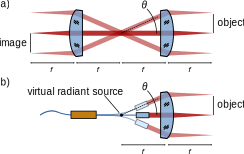
\includegraphics[width=\columnwidth]{figures/30_DesignSimulation/fps.pdf}
      \caption{\textbf{a)} Illustration of a classical telecentric system. The height of the object is translated into an angle $\theta$ in the collimated region between the two lenses. This angle is again translated into a corresponding image height by the second lens. \textbf{b)} Illustration of the OCT beam path using a fiber scanner in first resonance mode without micro prism and BS. The movement of the GRIN lens due to the fiber scanner and the distance between the GRIN lens and the focusing lens creating the same optical behavior as it can be observed in a classical object sided telecentric system. \textbf{c)} Nomenclature used in this work.}
      \label{fig:fps}
\end{figure}

For the scanner to work as a Fourier plane scanner, at any point of the oscillation the output beam from the GRIN lens should point to a fixed virtual radiant source. This is fulfilled if the bending shape of the scanner is linear with the amplitude and thus, the ratio of the GRIN lens angle to its vertical displacement is kept constant $ y = d \cdot \tan \theta \simeq d \cdot \theta \Rightarrow \frac{\theta}{y} = const $ (refer to Figure \ref{fig:radiant}).

\begin{figure}[h!]\centering
      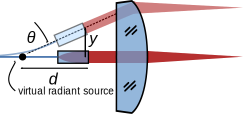
\includegraphics{figures/30_DesignSimulation/Mechanical/radiant.pdf}
      \caption{Schematic of the Fourier plane scanner at rest and at an arbitrary position with amplitude $\theta$. If the scanner behaves linearly, the output beam will appear to come from a fixed virtual radiant source regardless of the scanning amplitude.}
      \label{fig:radiant}
\end{figure}

\subsection{Component Selection}
Now that the basic design equations are obtained, it is possible to 

In a Fourier plane scanner, the numerical apertures and focal lengths of the scanning and objective lens are related by the diameter of the beam in the intermediate region between both lenses. Thus, following the schematic of Figure \ref{fig:fps}c, following geometrical optics relations are obtained: $d_\mathrm{beam} \simeq 2\cdot f_\mathrm{GRIN}\cdot \mathit{NA}_\mathrm{fiber}$ and $d_\mathrm{beam} \simeq 2 \cdot f_\mathrm{obj}\cdot \mathit{NA}_\mathrm{OCT}$. By combining them together the main design equation for the scanner appears:

\begin{equation}
f_\mathrm{GRIN} \cdot \mathit{NA}_\mathrm{fiber} = f_\mathrm{obj} \cdot \mathit{NA}_\mathrm{OCT}
\end{equation}

Note that these equations use a small angle approximation valid for small NA: \\ $\tan[	\sin^{-1}(\mathit{NA})] \simeq \mathit{NA} $. In this case, as any NA is smaller than 0.25, the error of this simplification is smaller than 2\%.

The design of the optical path for OCT is constrained by the commercial availability of the single mode fiber. The only one working in our wavelength range and with thinned cladding diameter (refer to Section \ref{sec:mechDesign}) is \textit{Thorlabs SM980G80}, with a diameter of \SI{80}{\micro\meter} and with $\mathit{NA_\mathrm{fiber}} = 0.18$ at \SI{1.330}{\micro\meter}. 

In order to collimate the output from the fiber without clipping the gaussian beam, a GRIN lens with an $\mathit{NA_{GRIN}}$ higher than $\mathit{NA_{fiber}}$ is neededf. A good fit from GRINTECH catalog is \textit{GT-LFRL-035-024-20-CC (1550)}, with an $\mathit{NA_\mathrm{GRIN}} = 0.20$ and $\mathit{f_\mathrm{GRIN}} = \SI{0.91}{\milli\meter}$. 

Now, by using the relation in Equation \ref{eq:fpsNA} we can design $f_\mathrm{objective}$ by choosing an adequate $\mathit{NA_\mathrm{OCT}}$. To preserve a high depth of field (DOF), allow enough space for the beamsplitter and a long working distance, a narrow $\mathit{NA_\mathrm{OCT}}$ is is preferred -- in the range of 0.020 - 0.025. By choosing an intermediate $\mathit{NA_\mathrm{OCT}}$ of 0.022, the focal length of the objective lens 
\begin{equation}
\mathit{f_\mathrm{obj}} = f_\mathrm{GRIN} \frac{\mathit{NA_\mathrm{fiber}}}{\mathit{NA_\mathrm{OCT}}}  = \SI{0.91}{\milli\meter} \frac{0.18}{0.022} = \SI{7.5}{\milli\meter}
\end{equation}
can be selected.

The field of view (FOV) of the OCT modality can be now calculated considering the maximum angular deflection of the GRIN lens in the tip of the scanning fiber by 
\begin{equation}
h_\mathrm{max} = f_\mathrm{obj}\cdot \tan  \theta_\mathrm{max} = \SI{7.5}{\milli\meter} \cdot \tan \SI{5}{\degree} = \SI{0.66}{\milli\meter} 
\end{equation}
equivalent to a FOV of \SI{1.2}{\milli\meter} for a $\theta_\mathrm{max} $ of $ \pm \SI{5}{\degree}$ (section \ref{sec:mechDesign}).


\subsection*{ZEMAX Simulation}

In order to validate the theoretical analysis of the optical design, we proceeded to a raytracing simulation using ZEMAX. By modeling the fiber facet as the waist of a gaussian beam, using the GRIN lens model provided by the manufacturer and a geometrical model of the prism, beamsplitter and planoconvex lens, the schematic shown in Figure \autoref{fig:BS}a is obtained. 

\begin{figure}[h!]\centering
      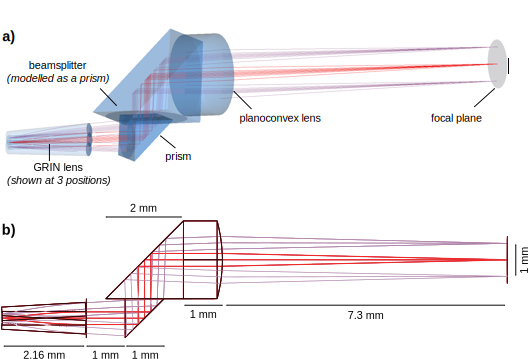
\includegraphics{figures/30_DesignSimulation/Optical/beamsplitterAll.pdf}
      \caption{\textbf{a)} 3D ZEMAX raytracing of the OCT beampath for the center (red rays) and marginal (purple rays) position of the GRIN lens.
      \textbf{b)} Cross section of a).}
      \label{fig:BS}
\end{figure}

The three overlapping rectangles on the left simulate the rest position (red) and maximum deflection (purple) of the GRIN lens. The gap between GRIN lens and prism is calculated so that the focus of the planoconvex lens coincides with the virtual radiant source of the scanner, and is numerically optimized to \SI{1}{\milli\meter}.

	Due to the low $\mathit{NA_\mathrm{OCT}}$ and the good optical quality of the GRIN and planoconvex lenses, the aberrations in this design are negligible and thus has an optical performance close to the diffraction limit. \autoref{fig:BSMTF} proves this behavior by comparing the MTF (Modulation Transfer Function) of an ideal optical system with the simulated MTF of the system which is described.

\begin{figure}[h!]\centering
      \includegraphics[width=10cm]{figures/30_DesignSimulation/Optical/beamsplitterMTF.png}
      \caption{(Change image)MTF curve of the multimode probe showing the...}
      \label{fig:BSMTF}
\end{figure}

\subsection{Minimization of backreflections}
After the geometrical simulation of the optical system is done, there is still an important factor to consider: the backreflections inside the probe. In Fourier Domain OCT, any backreflection coming from the probe increases the background intensity at the spectrometer, limiting its dynamic range. The consequences are higher noise, lower penetration depth and lower contrast of the resultant image. Thus any source of backreflections in the design should be carefully considered and minimized. The more important ones are marked in \autoref{fig:backreflections} and explained in the following list:

\begin{figure}[h!]\centering
      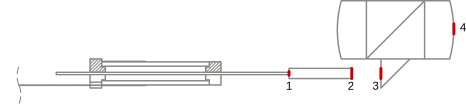
\includegraphics{figures/30_DesignSimulation/Optical/Backreflections/backreflections.pdf}
      \caption{Schematic of the multimodal probe showing the sources of backreflections (red).}
      \label{fig:backreflections}
\end{figure}

\begin{enumerate}

\item \textbf{Fiber-GRIN Interface:}
Starting from the proximal side, the fiber-GRIN interface consists of two parallel glass surfaces separated by a small gap. Although the beam is not collimated in this region, a small portion of light can be coupled back to the fiber. In order to minimize any backreflections, fiber and GRIN are glued together using a refractive-index-matched optical adhesive (\textit{NOA 76}, from \textit{Norland Products}). This way there is no glass to air interface and the maximum refractive index step is reduced to \SI{0.05}{}.
%Fiber 1.45670,NOA 1.51,GRIN 1.515 -> 275 ppm

\item \textbf{GRIN-Air Interface:}
The next interface is the distal facet of the GRIN lens. This is the most critical interface -- regardless of the scanning angle, it exhibits normal, collimated light incidence. To avoid this problem without resorting to delicate and expensive antireflection coatings (ARC), the GRIN lens is manufactured with a \SI{1}{\degree} tilted exit facet. According to geometrical optics, this tilt induces a vertical shift in the position of the backreflected focal point
\begin{equation}
\Delta y = f \tan(2\alpha)
\end{equation}

which is in this implementation equates to $\SI{0.91}{\milli\meter} \cdot \tan (\SI{2}{\degree}) = \SI{31}{\micro\meter}$.

The result is visible in the simulation from Figure \ref{fig:tilt}: the backreflected light is focused back with a \SI{31}{\micro\meter} offset, therefore missing the core of the fiber -- which has a diameter inferior to \SI{5}{\micro\meter}.

\begin{figure}[h!]\centering
      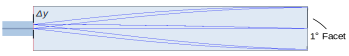
\includegraphics[width=10cm]{figures/30_DesignSimulation/Optical/backreflection.pdf}
      \caption{Simulation of backreflected light upon the distal end of a GRIN lens with a \SI{1}{\degree} tilted facet.}
      \label{fig:tilt}
\end{figure}

\item \textbf{Air-Prism Interface:} Due to collimated incidence, this interface can produce backreflections, but only in the resting position of the GRIN lens, when the free end of the GRIN lens is pointing perpendicular to the surface of the prism. To minimize reflections in this situation it is possible to resort to anti-reflection coatings in the facet of the prism. 

\item \textbf{Objective Lens - Air Interface:} After the prism, the beamsplitter and objective lens are cemented together, making any backreflections negligible. The objective lens has an interface with air, but has an anti-reflection coating on this surface. Furthermore, due to the curved surface of this lens, the backreflected light won't be focused back in the single mode fiber significantly.
\end{enumerate}

Taking these considerations into account, the backreflections were kept below 0.02\% in all the manufactured probes.

\subsection{Single Modality Probe}
As stated in the Design Overview, in order to independently test the behavior of the OCT scanner and optics, a single modality probe was fabricated as a demonstrator. Its optical design, depicted in \autoref{fig:single}, emulates the multimodal design from \autoref{fig:BS} by unfolding the optical path. The main difference is the lack of the prism and beamsplitter and the orientation of the planoconvex lens, which is now with its convex surface facing the GRIN lens to reduce the backreflections.

\begin{figure}[h!]\centering
      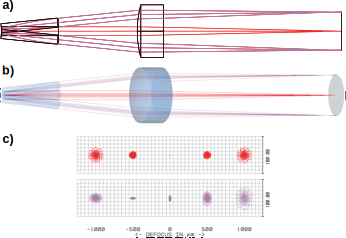
\includegraphics{figures/30_DesignSimulation/Optical/singleAll.pdf}
      \caption{\textbf{a)} 3D ZEMAX raytracing of the OCT beampath for the center (red rays) and marginal (purple rays) position of the GRIN lens in the single modality demonstrator.
      \textbf{b)} Cross section of a).}
      \label{fig:single}
\end{figure}

The equivalence of both systems is reaffirmed by the similarity of their MTF. Again, the simulated MTF from \autoref{fig:singleMTF} indicates that the single modality demonstrator is diffraction-limited.

\begin{figure}[h!]\centering
      \includegraphics[width=10cm]{figures/30_DesignSimulation/Optical/beamsplitterMTF.png}
      \caption{(Change image)MTF curve of the multimode probe showing the...}
      \label{fig:singleMTF}
\end{figure}

Due to these similarities, it is expected that any experimental result obtained with the demonstrator could be easily transferred to the behavior of the bimodal probe.

\subsection{Simulated Optical Performance of the demonstrator}

Table \ref{tab:simRes} summarizes the theoretical and simulated optical performance of the OCT microscope in both single modality and multimodality configurations.

\begin{table}[h!]\centering
	\begin{tabular}{rl}\\
		\hline
     	\textbf{Single mode fiber NA} & 0.18 \\ 
		\textbf{GRIN lens NA} & 0.2 \\ 
		\textbf{GRIN lens focal length} & \SI{0.91}{\milli\meter} \\ 
		\textbf{Planoconvex lens focal length} & \SI{7.5}{\milli\meter} \\ 
		\textbf{Distal Side NA} & 0.022 \\ 
		\textbf{Working Distance} & \SI{7.3}{\milli\meter} \\ 
		\textbf{Field of View} & \SI{1.2}{\milli\meter} \\ 
		\textbf{Depth of Field} & \SI{3.4}{\milli\meter} \\ 
		\textbf{Lateral Resolution} & \SI{43}{\micro\meter} \\ 
		\hline
	\end{tabular} 
    \caption{Simulated optical performance and characteristics of OCT modality. All resolution values follow the Rayleigh convention.}
    \label{tab:simRes}
\end{table}


%%*****************************************************************************

\section{Mechanical Design}
\label{sec:mechDesign}
%%*****************************************************************************

The fiber scanner uses resonance to amplify the subtle movement of the piezoelectric tube (in the order of $\pm \SI{3}{\micro\meter}$) into a big displacement and angular deflection of the GRIN lens (in the order of $\pm \SI{350}{\micro\meter}$ and  $\pm \SI{5}{\degree}$). Therefore, its geometrical and mechanical characteristics fully define the operating frequency range, and with it, constrain the way we can sample and acquire the final image.

\begin{figure}[h!]\centering
      \includegraphics[width=10cm]{figures/30_DesignSimulation/Mechanical/spiralScanning.pdf}
      \caption{Movement of the laser spot through time (red) and acquired points (black) during spiral scanning.}
      \label{fig:spiralScanning}
\end{figure}

As a resonant system, the movement of the scanning fiber is constrained to harmonic oscillations with a frequency close to $f_{resonance}$. Thus, the number of sample points $N_{T}$ that can be acquired in period $T$ depend on the resonant frequency of the scanner and the sampling frequency of the OCT system:

\begin{equation}
N_{T} = \frac{f_{sampling}}{f_{resonance}}
\label{eq:nT}
\end{equation}

As OCT systems have a relatively small sampling frequency ($\pm$\SI{100}{\kilo\hertz}), we need to decrease the resonant frequency below \SI{1}{kHz} to achieve more than 100 points per sampling period. The following paragraphs describe how to calculate and reduce this frequency.

\subsection{Resonant frequency calculation}
Following Euler Bernoulli theory, the spring constant for a fixed-free, point loaded cantilever is given by Equation \ref{eq:EB}, considering that the moment of inertia of the cylindrical fiber is given by $I_{fiber} = \frac{\pi}{4} r^4$.


\begin{equation}
K_{cantilever} = \frac{3 E I}{L^3} = \frac{3 \pi}{4} \frac{E_{fiber} r_{fiber}^4}{L^3}
\label{eq:EB}
\end{equation}

\begin{figure}[h!]\centering
      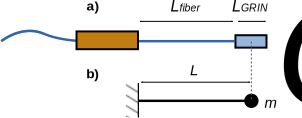
\includegraphics{figures/30_DesignSimulation/Mechanical/EB.pdf}
      \caption{\textbf{a)} Drawing of the piezoelectricscanner: piezoelectric tube, fiber and GRIN lens. 
      \textbf{b)} Simplified mechanical diagram, }
      \label{fig:EB}
\end{figure}

Approximating the fiber - GRIN assembly as a weightless, flexible, fixed-free cantilever and concentrating the weight of the GRIN lens in its center of gravity (Figure \ref{fig:EB}), we can estimate the resonant frequency of the scanner by applying the ideal mass-spring harmonic resonator equation for the first resonant mode (Eq. \ref{eq:fres}) \footnote{In order to assess the error of this approximation, we repeated the calculation of the resonant frequency using the method described in \cite{Huo2010}. In the plotted range, the error was smaller than 2\%.}. 

\begin{equation}
f_{res} = \frac{1}{2 \pi} \sqrt{\frac{K_{cantilever}}{m_{\mathit{GRIN}}}} 
\label{eq:fres}
\end{equation}

As we can observe from equation \ref{eq:EB} and \ref{eq:fres}, the resonance frequency increases quadratically with the diameter of the fiber. Therefore, by choosing a fiber with \SI{80}{\micro\meter} instead of the standard \SI{125}{\micro\meter}, the resonance frequency can be lowered from \SI{1900}{\hertz} to \SI{770}{\hertz} for a \SI{4.5}{\milli\meter} scanner.

The resonant frequency of a cantilever formed by a \SI{80}{\micro\meter} fused silica fiber with the chosen GRIN lens is computed in Figure \ref{fig:freq}.

\begin{figure}[h!]\centering
      \includegraphics[width=10cm]{figures/30_DesignSimulation/Mechanical/fres.pdf}
      \caption{Resonant frequency as a function of the scanning tip length (fiber + GRIN lens).}
      \label{fig:freq}
\end{figure}

As the scanner is buried in a \SI{1}{\milli\meter} channel, the maximum displacement of the GRIN lens is limited to $\pm\SI{325}{\micro\meter}$. Within that small displacement we want to achieve the maximum angular deflection of the GRIN lens to maximize the FOV, what can be achieved by using shorter fiber lengths. This shows a trade-off with the density of sampling $N_{T}$ -- which is increased with longer fiber lengths. To balance those terms, we chose a a total scanner length of \SI{4.5}{\milli\meter}, with characteristics summarized in Table \ref{tab:mech}.

\begin{table}[h!]\centering
	\begin{tabular}{rl}\\
		\hline
		\textbf{Total scanner length} & \SI{4.5}{\milli\meter} \\ 
		\textbf{Resonant Frequency} & \SI{770}{\hertz} \\ 
		\textbf{Max. angular deflection} & \SI{5}{\degree} \\ 
		\hline
	\end{tabular} 
    \caption{Mechanical charactaristics.}
    \label{tab:mech}
\end{table}

\subsection{COMSOL simulation}
In order to validate the theoretical analysis of the previous section, we performed a multiphysics FEM analysis using COMSOL. For that matter, the piezoelectricactuator was modeled as a radially polarized piezoelectric material (\textit{PIC 151}) and the rest of the structure as elastic material. The excitation voltage is a sinusoidal symmetrical potential between the top and bottom electrodes of the tube. As the system undergoes small deflections, it is simulated assuming linear behavior \cite{Fertis2006}.

The first step is to simulate the resonant frequency of the system. Performing an \textit{Eigenfrequency} study, we obtain a first mode resonance at \SI{762}{\hertz}, which closely matches our analytical estimation (\SI{770}{\hertz}. The mode shape is shown in Figure \ref{fig:defle}.

\begin{figure}[h!]\centering
      \includegraphics[width=10 cm]{figures/30_DesignSimulation/Mechanical/deflection.pdf}
      \caption{COMSOL simulation of the total deflection in at resonance (\SI{762}{\hertz}).}
      \label{fig:defle}
\end{figure}

Note that, as the system is working at its resonance, it is very difficult to simulate the oscillation amplitude, as it depends on its damping factor which should be obtained experimentally. Thus, for the simulation, this value was chosen to fit the expected deflection. 

Thanks to the multiphysics simulation, we can also check the electric field distribution inside the piezoelectric tube. As can be seen in Figure \ref{fig:field}, for a symmetrical actuation in the left and right electrodes with a voltage of $\pm \SI{75}{\volt}$, most of the volume under those electrodes experiences a field magnitude close to the expected theoretical value $E=U/d = \SI{75}{\volt}/\SI{150}{\micro\meter} = \SI{500}{\volt/\meter}$, which is under the safe operating field of \textit{PIC 151}: $ +\SI{1000}{\volt/\meter}$ to $ -\SI{700}{\volt/\meter}$. Only some fringe areas exceed these values, which could become depolarized with time.
\begin{figure}[h!]\centering
      \includegraphics[width=10 cm]{figures/30_DesignSimulation/Mechanical/field.png}
      \caption{Magnitude of the electrical field [\SI{}{\kilo \volt / \meter}] inside a cross-section of the piezoelectric tube with an excitation voltage of $\pm \SI{75}{\volt}$}.
      \label{fig:field}
\end{figure}





